\documentclass{article}

\usepackage[utf8]{inputenc}
\usepackage[T1]{fontenc}
\usepackage[francais]{babel}
\usepackage{titling}
\setlength{\droptitle}{-3cm}
\usepackage{graphicx} 

\title{Planification et gestion de projet}
\author{CAROT Axel, ARISOY Ivan Can, \\ DARDE Guilhem, NDJINGA NDJINGA Anta Claude}
\date{\today}

\begin{document}
\maketitle

\section{Élection du «Team Leader»}
Après une concertation, nous avons décidé d'élire DARDE Guilhem en tant que TEAM Leader. Son rôle sera de :
\begin{itemize}
    \item La coordination des efforts synergiques de tous les membres de l’équipe.
    \item L'assistance dans la distribution équitable des tâches et des responsabilités, en tenant compte des compétences individuelles et des centres d'intérêt.
    \item L'organisation des rôles au sein de l'équipe de manière démocratique et inclusive.
    \item L'assurance d'une communication fluide et transparente entre tous les membres de l'équipe.
    \item Le suivi rigoureux de l'avancement des sous-tâches et l'anticipation proactive des obstacles éventuels.
    \item L'insufflation d'une motivation constante au sein du groupe.
\end{itemize}

\section{Planification des tâches et stratégie}

\subsection{Sélection d'un outil de gestion de projet : Trello}
L'utilisation de Trello dans des projets antérieures et sa simplicité ont été les facteurs décisifs dans le choix de cet outil. De plus, cet outil offre  des visualisations graphiques qui enrichissent la représentation de notre planning. (tableau, chronogramme, tableau de bord)

\begin{figure}[h]
    \centering
    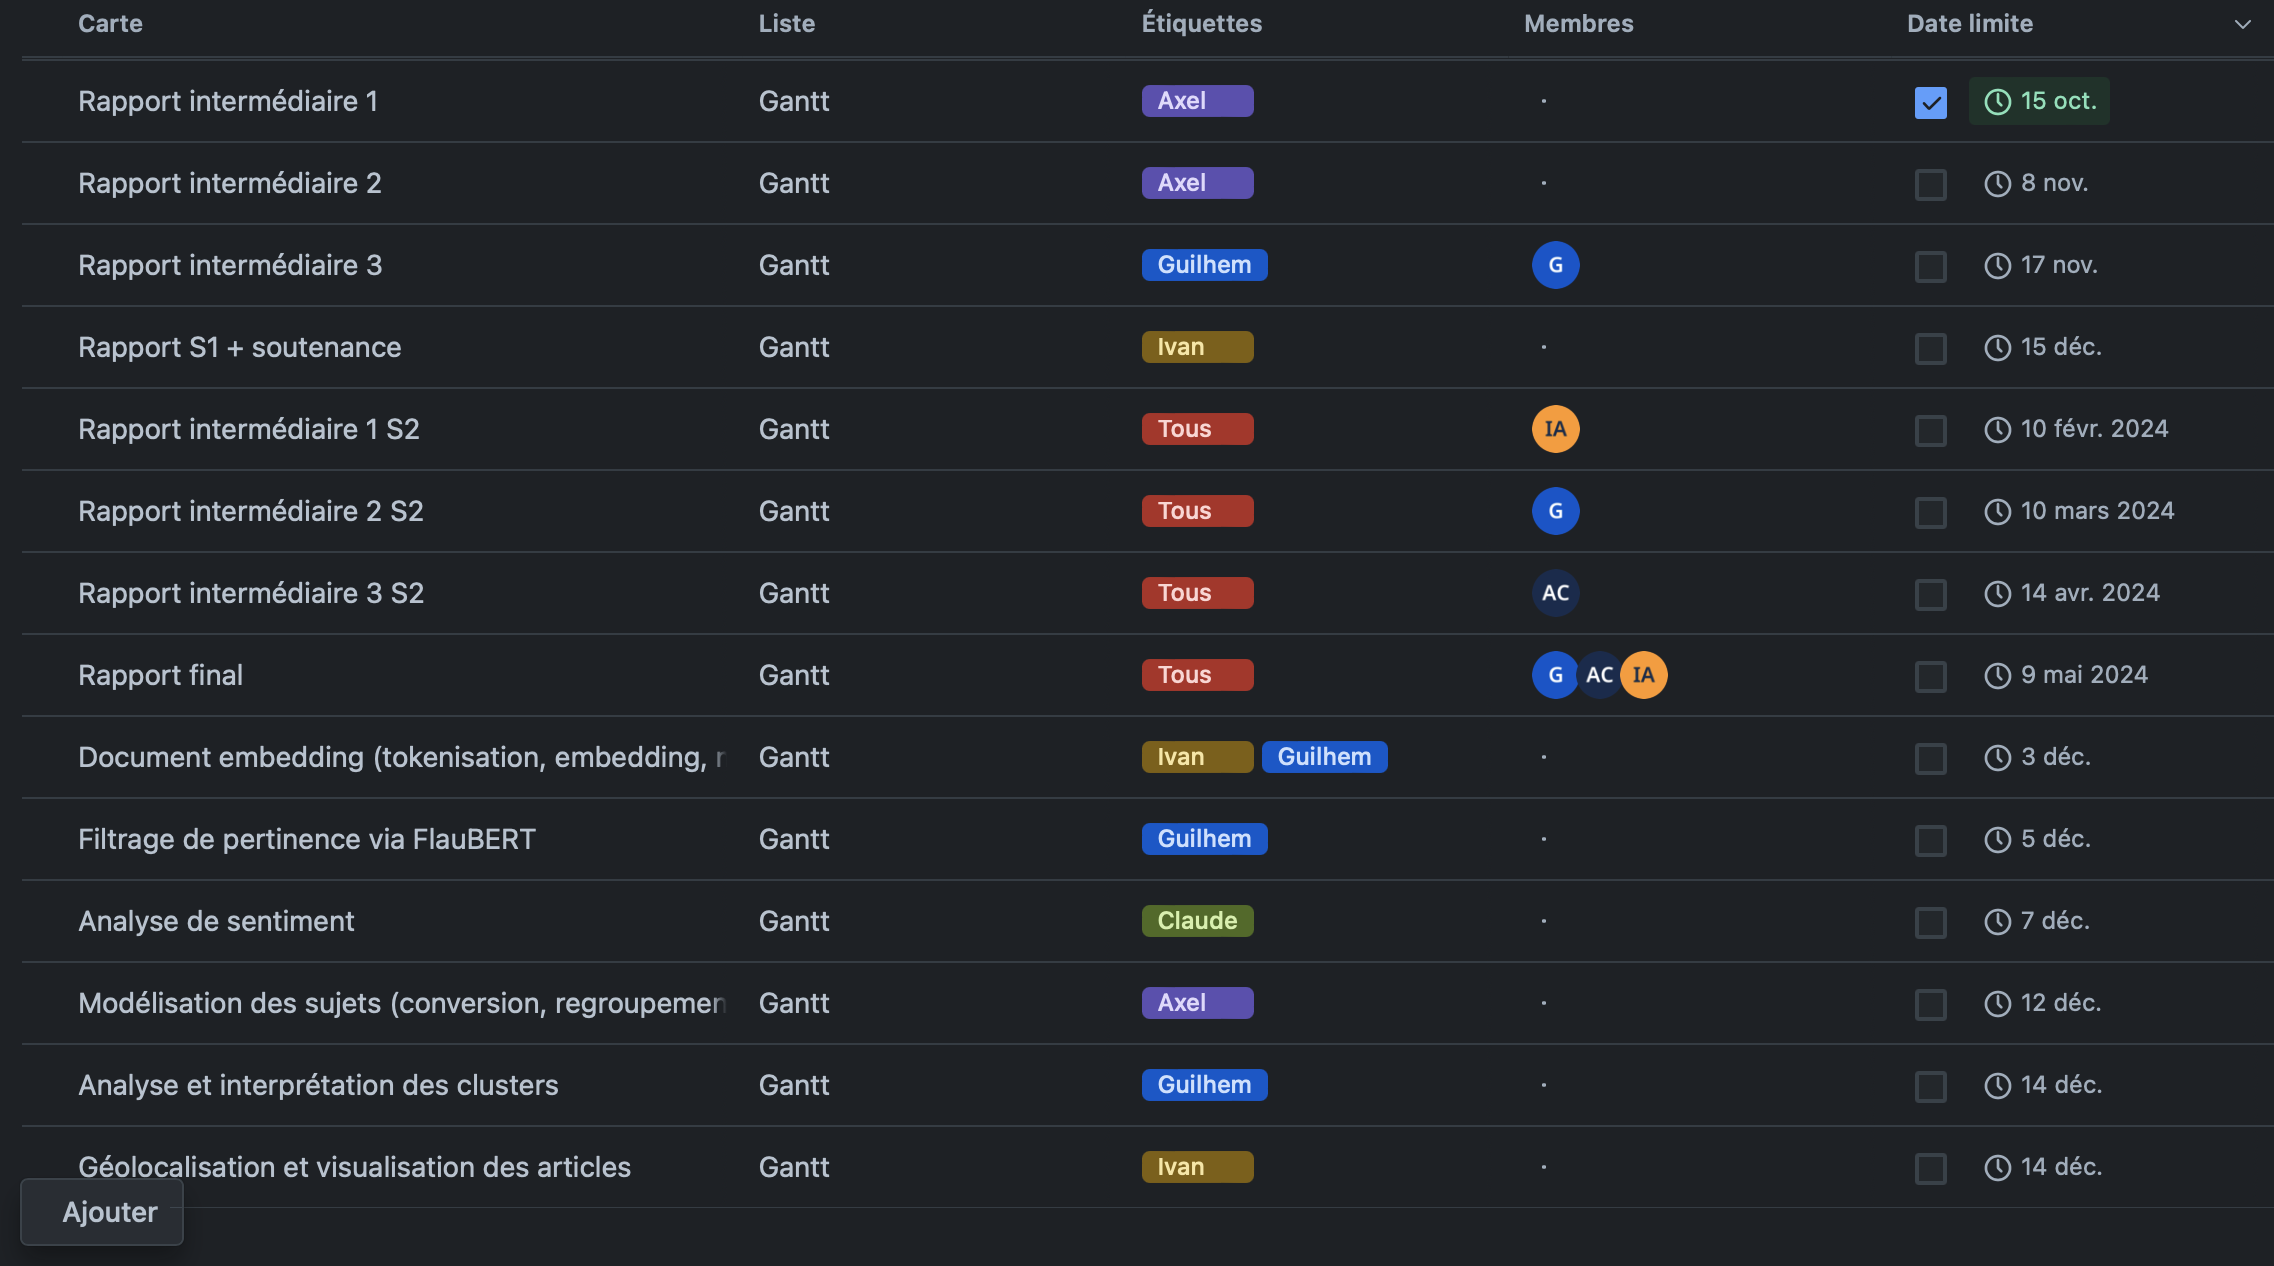
\includegraphics[width=0.7\textwidth]{tableur.png}
    \caption{Tableur}
    \label{fig:mon_image}
\end{figure}
\vspace{5cm}

De plus, Trello dispose de la fonctionnalité calendrier qui nous permet de synchroniser nos rendez-vous, de fixer les dates de nos débriefings et de suivre nos diverses échéances. Cette fonctionnalité nous dispense donc de l'utilisation d'un autre outil de gestion comme Google Agenda. 

\begin{figure}[h]
    \centering
    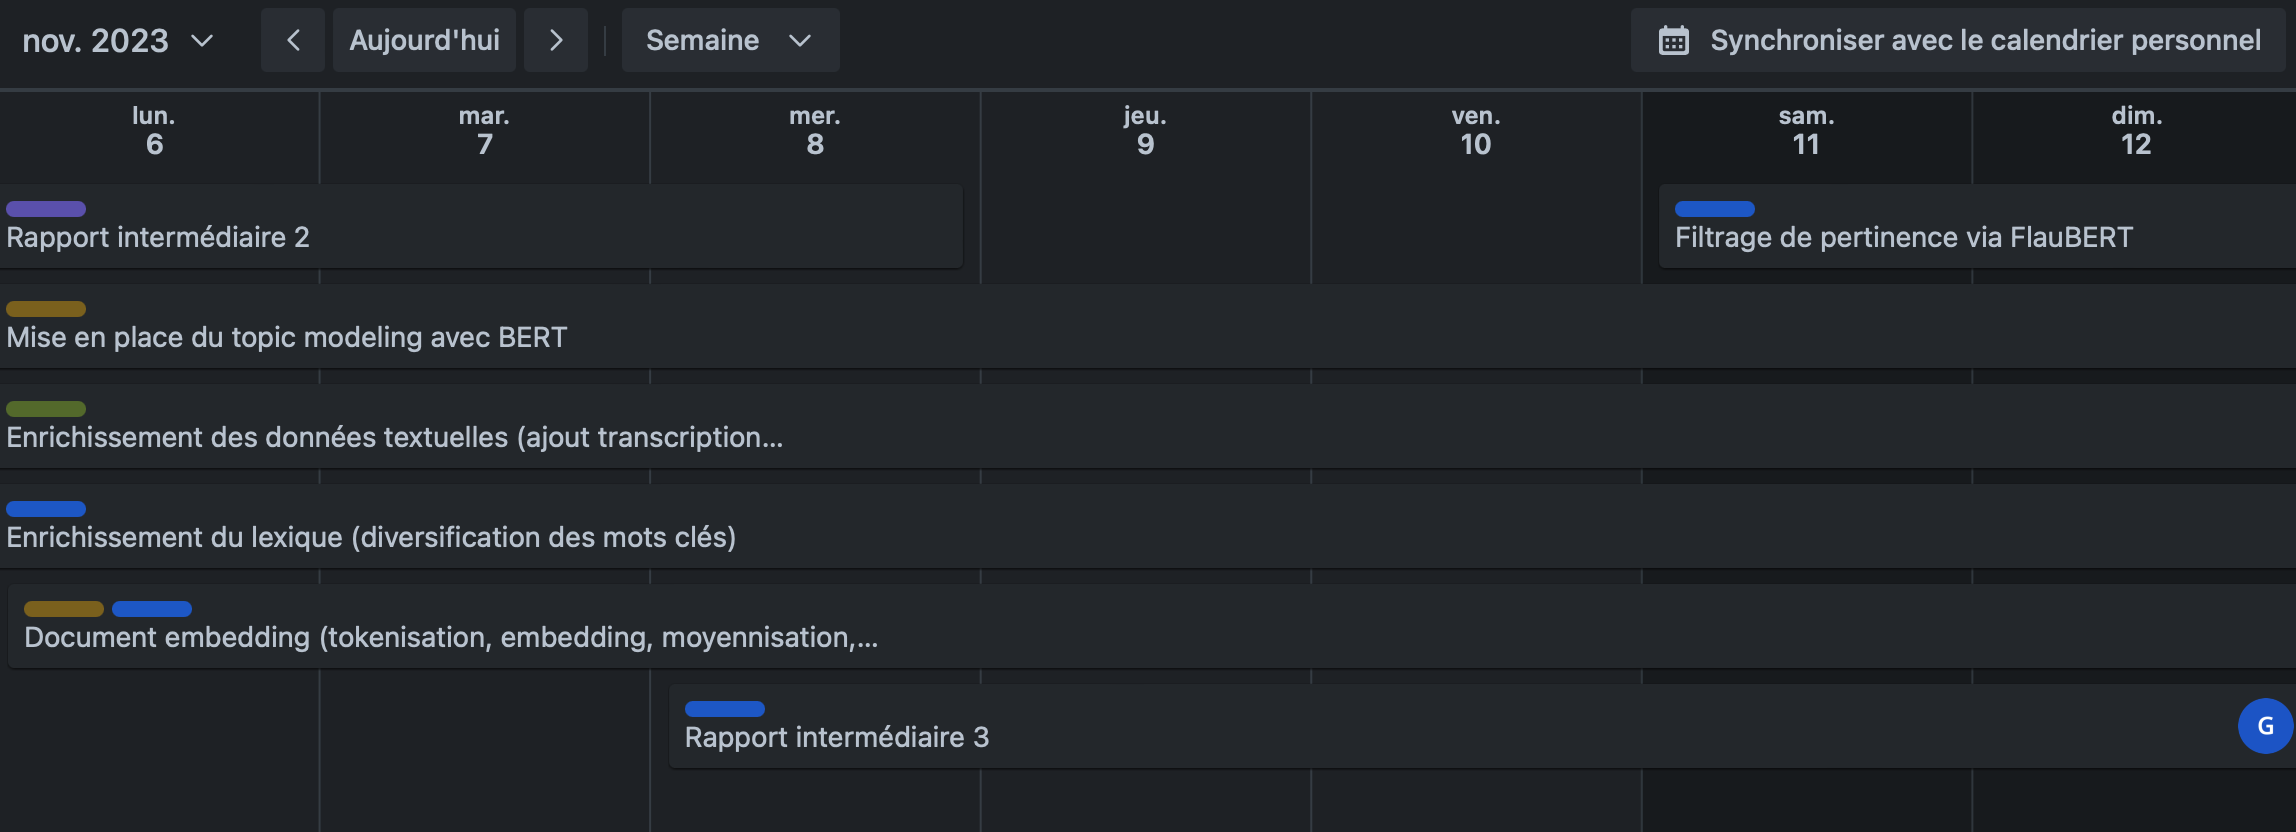
\includegraphics[width=0.8\textwidth]{calendrier.png}
    \caption{Calendrier}
    \label{fig:mon_image}
\end{figure}

\subsection{Stratégie et Planification des tâches}

Dans le cadre de l'élaboration de notre stratégie d'organisation, notre premier pas a été l'examen approfondi de la documentation fournie, afin de maîtriser la théorie sous-jacente aux différentes étapes du pipeline pour l'analyse spatio-temporelle des données textuelles. Ce pipeline a été établis par nos commanditaires et les étapes principales sont les suivantes : 
\begin{itemize}
    \item Acquisition des données
    \item Traitement du texte
    \item La sélection d'articles pertinents comportant des termes clés spécifiques (word embedding)
    \item Modélisation de sujets (LDA)
    \item Développement de l'indicateur TXT-FS
    \item L'application et la mise en œuvre concrète des données traitées. \\
\end{itemize}

Nos commanditaires ont exprimé le désir d'apporter des améliorations au pipeline existant. Nous avons, en conséquence, attribué les missions d'amélioration suivantes en adéquation avec nos préférences respectives :
\begin{itemize}
    \item L'enrichissement de la base de données initiale (comprenant des articles, des données de presse, etc.).
    \item L'élargissement et la révision du lexique de mots-clés.
    \item Le remplacement des techniques de modélisation de sujets existantes par des modèles telles que Bert (modèle de langage de grande envergure), CamemBERT, et le filtrage de pertinence inspiré de FlauBERT. Prise en compte de la temporalité. 
    \item L'analyse de sentiment et pertinence. 
    \item L'expansion des données d'entrée grâce à l'intégration de contenus radiophoniques. \\
\end{itemize}

\begin{figure}[h]
    \centering
    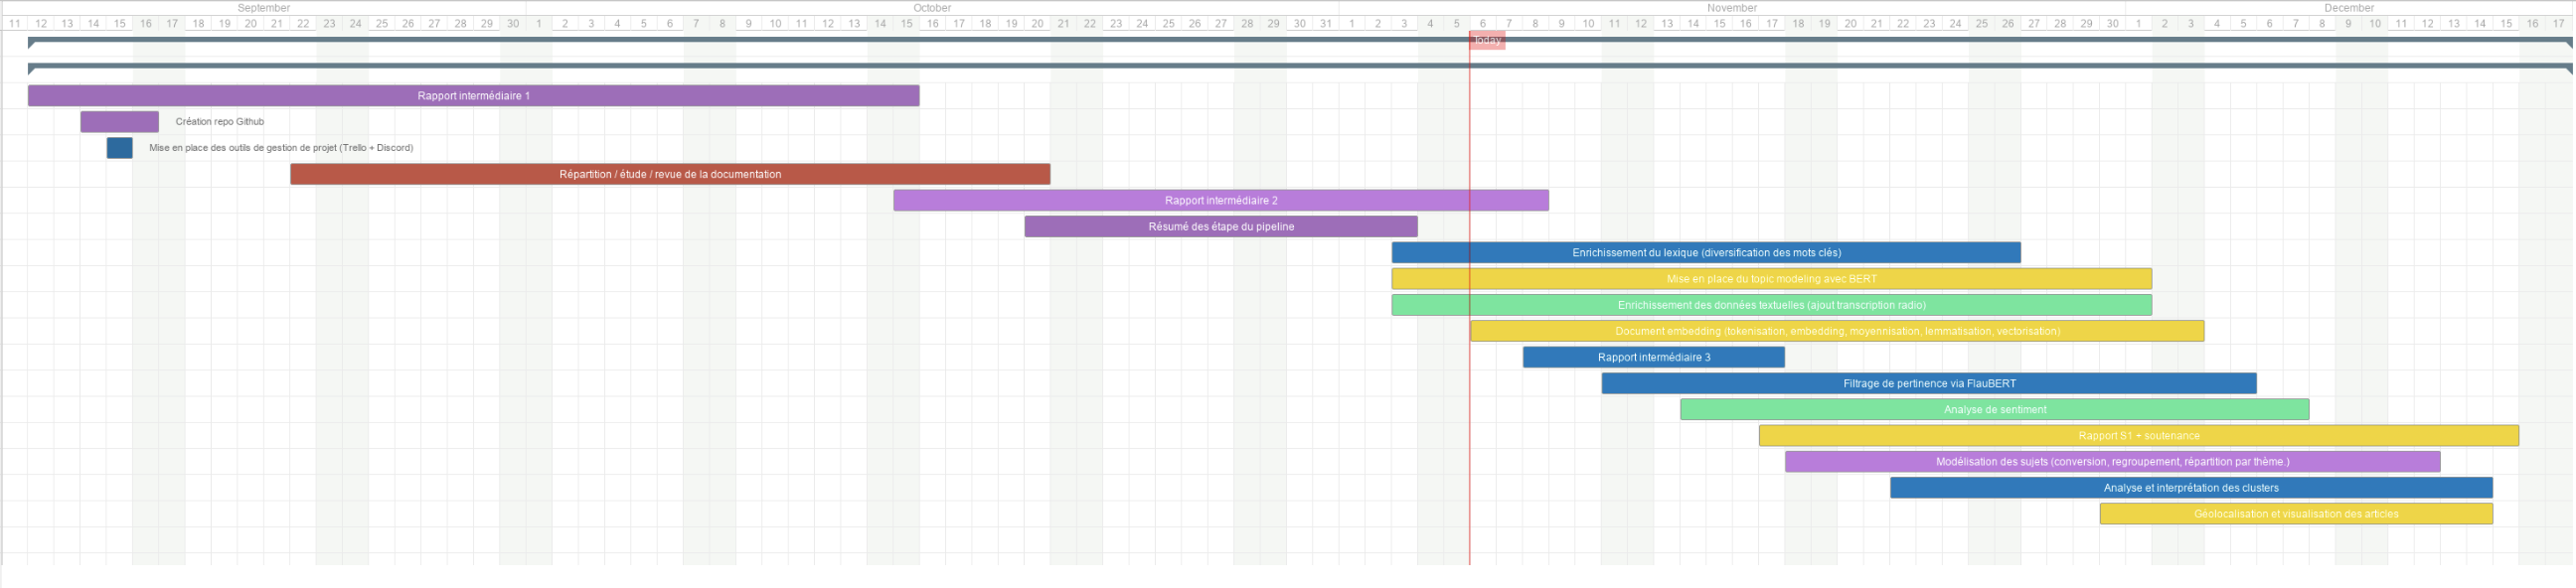
\includegraphics[width=1\textwidth]{gantt.png}
    \caption{Diagramme de Gantt }
    \label{fig:mon_image}
\end{figure}

Les couleurs sur le diagramme représentent les membres de l'équipe : Violet : Axel, Bleu : Guilhem, Jaune : Ivan, Vert : Claude, et Rouge : les tâches réalisées en groupe. \\

Nous avons planifié les tâches en adéquation avec la séquence opérationnelle du pipeline, car nous ne savons pas encore si certaines tâches peuvent être exécutées en parallèle, en particulier celles liées au remplacement des techniques de modélisation de sujets (topic modeling). Il est possible que certaines tâches dépendent directement des résultats d'autres tâches. Néanmoins, cette interdépendance ne s'applique pas à toutes les activités, comme l'enrichissement des données d'entrée, la mise à jour du lexique, ou encore la transcription des données issues de la radio.

\end{document}
